\documentclass[12pt]{report}
\usepackage[utf8]{inputenc}
\usepackage{amsmath}
\usepackage{amsfonts}
\usepackage{amssymb}
\usepackage{graphicx}
\usepackage{adjustbox}
\usepackage{array}
\usepackage{ragged2e}
\usepackage{booktabs}
\usepackage{multirow}
\usepackage{tikz}
\usepackage{pgfplots}
\usepackage{xcolor}
\usepackage{graphics}
\usetikzlibrary{positioning,shapes,arrows}


\begin{document}

%change k to m...

\begin{figure}[h!]
\scalebox{1}{
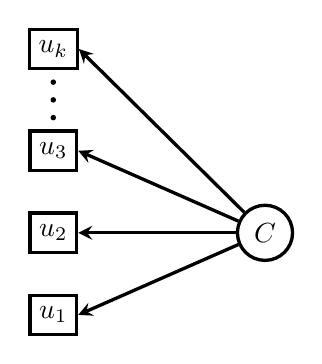
\begin{tikzpicture}[
  transform shape, node distance=2cm,
  roundnode/.style={circle, draw=black, very thick, minimum size=7mm},
  squarednode/.style={rectangle, draw=black, very thick, minimum size=5mm},
  dotnode/.style={fill,inner sep=0pt,minimum size=2pt,circle} % <- this is new
]

%Nodes
\node[roundnode] (latent) {$C$};
\node[squarednode, left=2cm of latent] (u2) {$u_2$}; 
\node[squarednode, above=0.5cm of u2]    (u3) {$u_3$};
\node[squarednode, below=0.5cm of u2]    (u1) {$u_1$};
\node[squarednode, above=0.75cm of u3]    (uk) {$u_k$};

%Arrows 
\draw[->,very thick,-stealth] (latent) -- node[]{} (u1.east);
\draw[->,very thick,-stealth] (latent) -- node[]{} (u2.east);
\draw[->,very thick,-stealth] (latent) -- node[]{} (u3.east);
\draw[->,very thick,-stealth] (latent) -- node[]{} (uk.east);

\path (u3) --
  node[dotnode,pos=0.2]{}
  node[dotnode,pos=0.5]{}
  node[dotnode,pos=0.8]{}
  (uk);
\end{tikzpicture}}
\hspace{0.8cm}
\scalebox{1}{
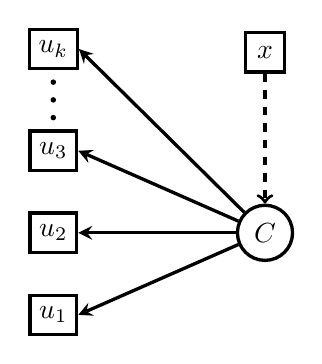
\begin{tikzpicture}[
  transform shape, node distance=2cm,
  roundnode/.style={circle, draw=black, very thick, minimum size=7mm},
  squarednode/.style={rectangle, draw=black, very thick, minimum size=5mm},
  dotnode/.style={fill,inner sep=0pt,minimum size=2pt,circle} % <- this is new
]

%Nodes Picture 2
\node[roundnode] (latent) {$C$};
\node[squarednode, left=2cm of latent] (u2) {$u_2$}; 
\node[squarednode, above=1.65cm of latent] (x) {$x$};
\node[squarednode, above=0.5cm of u2]    (u3) {$u_3$};
\node[squarednode, below=0.5cm of u2]    (u1) {$u_1$};
\node[squarednode, above=0.75cm of u3]    (uk) {$u_k$};

%Arrows 
\draw[->,very thick,-stealth] (latent) -- node[]{} (u1.east);
\draw[->,very thick,-stealth] (latent) -- node[]{} (u2.east);
\draw[->,very thick,-stealth] (latent) -- node[]{} (u3.east);
\draw[->,very thick,-stealth] (latent) -- node[]{} (uk.east);
\draw[->,very thick,dashed] (x) -- node[]{} (latent.north);

\path (u3) --
  node[dotnode,pos=0.2]{}
  node[dotnode,pos=0.5]{}
  node[dotnode,pos=0.8]{}
  (uk);
\end{tikzpicture}}
\hspace{0.8cm}
\scalebox{1}{
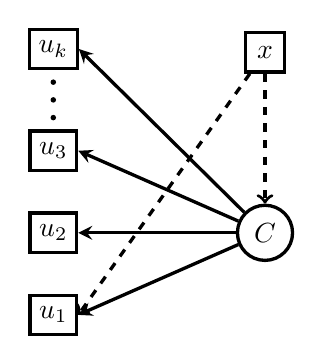
\begin{tikzpicture}[%Third Picture
  transform shape, node distance=2cm,
  roundnode/.style={circle, draw=black, very thick, minimum size=7mm},
  squarednode/.style={rectangle, draw=black, very thick, minimum size=5mm},
  dotnode/.style={fill,inner sep=0pt,minimum size=2pt,circle} % <- this is new
]

%Nodes Picture 3
\node[roundnode] (latent) {$C$};
\node[squarednode, left=2cm of latent] (u2) {$u_2$}; 
\node[squarednode, above=1.65cm of latent] (x) {$x$};
\node[squarednode, above=0.5cm of u2]    (u3) {$u_3$};
\node[squarednode, below=0.5cm of u2]    (u1) {$u_1$};
\node[squarednode, above=0.75cm of u3]    (uk) {$u_k$};

%Arrows 
\draw[->,very thick,-stealth] (latent) -- node[]{} (u1.east);
\draw[->,very thick,-stealth] (latent) -- node[]{} (u2.east);
\draw[->,very thick,-stealth] (latent) -- node[]{} (u3.east);
\draw[->,very thick,-stealth] (latent) -- node[]{} (uk.east);
\draw[->,very thick,dashed] (x) -- node[]{} (latent.north);
\draw[->,very thick,dashed] (x) -- node[]{} (u1.east);


\path (u3) --
  node[dotnode,pos=0.2]{}
  node[dotnode,pos=0.5]{}
  node[dotnode,pos=0.8]{}
  (uk);
\end{tikzpicture}}
\caption{M1} \label{fig:M1}
\end{figure}



\begin{figure}
 \begin{center}
    \begin{tikzpicture}[scale=1.05]
    \begin{axis}[
    xlabel={Latent response $u^{*}$},
    ylabel={Density}]
    \addplot[color=black]{ ((exp(-x)))/((1+exp(-x)^2) };
    \end{axis}
    \draw [dashed] (1.7,0) -- (1.7, 5.5);
    \draw [dashed] (4,0) -- (4,5.5)
    \end{tikzpicture}
    \caption{M1} \label{}
 \end{center}
\end{figure}


\end{document}
